\chapter{Atividades Desenvolvidas}\label{sec:ativ_desenvolvidas}
Nesta seção são descritas, em detalhes, as principais atividades realizadas para a condução deste projeto.

\section{Estudo sobre usabilidade e acessibilidade}\label{sec:estudos_usab_acess} 

Segundo a Lei 10.098, de 19 de dezembro de 2000 da Legislação Brasileira\footnote{\url{https://www2.camara.leg.br/legin/fed/lei/2000/lei-10098-19-dezembro-2000-377651-publicacaooriginal-1-pl.html}}, a acessibilidade é a possibilidade e condição de alcance para utilização, com segurança e autonomia, dos
espaços, mobiliários e equipamentos urbanos, das edificações, dos transportes e dos sistemas e meios de comunicação por pessoa portadora de deficiência ou com mobilidade reduzida. 

De modo complementar, \cite{torres2002acessibilidade} diz que acessibilidade é um processo dinâmico, associado não só ao desenvolvimento tecnológico, mas principalmente ao desenvolvimento da sociedade. Em geral, está associada a pessoas com deficiências físicas ou psicológicas, idosos ou grupos excluídos; este último mais bem relacionado com o termo \textit{inclusão}. 

Embora a acessibilidade não se restrinja ao meio digital, é essencial que esteja presente no mesmo. Corroborando com essa ideia, \cite{leew3c} afirma a importância da Web ser utilizável por qualquer um, independente de capacidades individuais ou deficiências. No cenário atual, isso também se aplica ao uso de aplicativos em dispositivos móveis.

Apesar da elicitação da acessibilidade no campo jurídico, social e meio digital, faz-se necessário um foco adicional ao campo educacional. De acordo com \cite{Bine2018DigitalIT}, a educação inclusiva se tornou uma das questões mais desafiadoras dos sistemas educacionais atuais. Isso ocorre em parte pela falta de preparo de professores e deficiência de material.

Atrelada à acessibilidade deve estar a usabilidade que, segundo \cite{nielsenPrioritizingWebUsability},
é o atributo relacionado a quão fácil é usar algo. Mais especificamente, refere-se a quão rápido pessoas podem aprender a usar uma ferramenta, quão eficientes são enquanto a utilizam, quão memorável é, quão propenso a erros e o quanto as pessoas gostam de utilizar; deve-se tornar a utilização fluida. É interessante destacar que existe uma frase entre desenvolvedores que diz: ``não faça o usuário pensar'' baseada no livro \textit{Don't make me think} \citep{steveDont2005}. O objetivo é tornar o processo intuitivo o suficiente a ponto de ser considerado natural.
Ainda, é essencial analisar fatores como capacidade de aprendizagem, a fim de que não seja necessário um aprendizado extra por parte do usuário para utilizar o sistema em questão.

No contexto em que se insere este trabalho isso se torna ainda mais essencial, uma vez que o público idoso enfrenta vários problemas relacionados à usabilidade em \textit{smartphones} \citep{dificuldadesIdosos} e principalmente à acessibilidade.

Ressalta-se que o objetivo principal do projeto é auxiliar o processo de ensino-aprendizagem de usuários idosos e o foco é no desenvolvimento de aplicações com base em requisitos pedagógicos e de acessibilidade.

\section{Estudo sobre aprendizagem móvel}\label{sec:estudos_ap_movel} 
Outra atividade realizada foi o estudo do conceito de aprendizagem móvel, bem como uma pesquisa sobre as principais funcionalidades presentes em aplicativos relacionados ao ensino de palavras cruzadas, tendo como público-alvo o usuário idoso.

\subsection{Visão geral}
Existem várias definições de \textit{m-learning}.
De acordo com \cite{Quinn2000}, \textit{m-learning} é um modelo de aprendizagem eletrônica (\textit{e-learning}) que utiliza equipamentos computadorizados: \textit{Palmtops}, dispositivos que rodam \textit{Windows Embedded Compact} e até um telefone celular.
Em 2011, \cite{hwang2011research} argumentaram que uma definição amplamente aceita de \textit{m-learning} é simplesmente ``usar tecnologias móveis para facilitar o aprendizado''. Dentre outras definições, a adotada para esse projeto é a de \cite{traxler2005defining}: qualquer fornecimento educacional onde a tecnologia dominante é portátil ou dispositivos \textit{palmtop}.

Todavia, independentemente da definição considerada, torna-se necessário analisar as vantagens e desvantagens de se utilizar dispositivos móveis no processo de ensino-aprendizagem. De acordo com \cite{RICHAMEHTA2016} destacam-se como vantagens: 

\begin{itemize}
    \item Tablets com anotações e e-books são mais leves e menos volumosos que mochilas cheias de papéis, livros e até laptops;
    \item É mais fácil acomodar dispositivos móveis em uma sala se comparado à computadores de mesa;
    \item Dispositivos móveis podem ser usados em qualquer lugar e em qualquer momento, como em trens, em casa, em hotéis; e isto tem um valor inestimável para a educação \citep{CarmaMaia2008}.
\end{itemize}

Porém, de acordo com \cite{RICHAMEHTA2016}, as seguintes desvantagens devem ser destacadas: 

\begin{itemize}
    \item Celulares pequenos limitam-se a quantidade e tipo de informação que pode ser exibida;
    \item Baterias precisam ser recarregadas regularmente, e dados podem ser perdidos caso não se faça o carregamento correto;
    \item É difícil usar gráficos que possuem movimento, especialmente em celulares pequenos.
\end{itemize}

Dessa forma, devido ao processo de envelhecimento, limitações e desafios podem ser potencializadas no caso de usuários idosos. Além disso, é necessário que as aplicações educacionais móveis levem em consideração propostas pedagógicas adequadas e específicas para esse público. Logo, é indispensável que o desenvolvimento dessas aplicações seja realizado de maneira clara e objetiva, possibilitando melhor aprendizagem por parte do idoso \citep{giubilei1993pedagogia}.

\subsection{Estudo sobre as principais funcionalidades do aplicativo}
\label{sec:estudo_funcionalidades_apps}

Diversos são os aplicativos que visam apoiar o processo de ensino-aprendizagem do usuário, seja por meio de jogos, vídeos ou outros materiais. 

Dessa maneira, alguns aplicativos (para diferentes públicos) foram analisados, a fim de verificar suas funcionalidades e propostas de aprendizagem e acessibilidade, de modo que essas pudessem ser adaptadas ou utilizadas para aplicações com foco no idoso.

\begin{description}

\item[Engaging congress]\footnote{\url{https://play.google.com/store/apps/details?id=com.iu.engagingcongress&hl=en}, \url{https://apps.apple.com/us/app/engaging-congress/id1309161238?ls=1}} \hfill \\
\textit{Enganging congress} (\autoref{fig:EngCong}) é um jogo interativo que visa explorar os princípios básicos de um governo representativo. Escolhe-se um tema e é exibido um vídeo. Jogos são incluídos no processo baseados no tema em questão. É importante destacar a atenção dos criadores em fazer o usuário compreender a tarefa; a todo momento é possível clicar no botão de dúvida. As principais funcionalidades são: (i) aprendizado por conteúdo em formato de áudio sobre o tema; (ii) perguntas relacionadas ao conteúdo passado; (iii) nota final após a conclusão dos exercícios; (iv) botões de dúvidas sempre presentes.

\begin{figure}[ht!]
\centering
    \caption{Telas do aplicativo \textit{Engaging Congress}}
    \label{fig:EngCong}
    \includegraphics[width=0.9\textwidth]{Figuras/engagingcongress.png}
    
    Fonte: Capturas de tela do aplicativo
\end{figure}

\item[Play PBS KIDS Games]\footnote{\url{https://apps.apple.com/us/app/pbs-kids-games/id1050773989}, \url{https://play.google.com/store/apps/details?id=org.pbskids.gamesapp&hl=pt_BR}} \hfill \\
O aplicativo \textit{Play PBS KIDS Games} (\autoref{fig:pbs}) visa a promoção da educação para crianças na fase de alfabetização (2 a 8 anos), contendo mais de 100 mini-jogos voltados para tal. As crianças são encorajadas a resolver desafios e aprimorar suas habilidades em ciências, matemática, letras e criatividade. O objetivo é impactar positivamente a vida de crianças por meio de mídia baseada em um currículo onde quer que elas estejam. O aplicativo ganhou duas premiações no ano de 2017, a saber Melhor aplicativo de jogos para Pré-Escola (\textit{Kidscreen Award Winner}) e o \textit{Parents' Choice Recommended Mobile App}. Os principais recursos são: (i) funcionamento offline; (ii) possibilidade de gerenciar a quantidade de memória que será consumida; (iii) obtenção de detalhes sobre desenhos da TV PBS Kids, como idade recomendada e objetivos de aprendizado para as crianças.

\begin{figure}[H]
\centering
    \caption{Telas do aplicativo \textit{Play PBS KIDS Games}}
    \label{fig:pbs}
    \includegraphics[width=0.6\textwidth]{Figuras/pbsKids.jpg}
    
    Fonte: Capturas de tela do aplicativo
\end{figure}

\item[Human Anatomy Atlas]\footnote{\url{https://apps.apple.com/br/app/human-anatomy-atlas-2020/id1117998129}, \url{https://play.google.com/store/apps/details?id=com.argosy.vbandroid&hl=pt_BR}} \hfill \\
O \textit{Human Anatomy Atlas} (\autoref{fig:humAtlas}) é um aplicativo criado por um time de especialistas em visualização biomédica. É direcionado ao ensino da anatomia do corpo humano com o foco em estudantes e professores, apesar de também ser utilizado em hospitais. Seus modelos em 3D promovem uma fidelidade às estruturas humanas reais, sendo possível rotacionar e dissecar órgãos e partes do corpo. Possui recursos como : (i) interatividade com estruturas 3D; (ii) mais de 1000 questões para testes em assuntos; (iii) visualização de anatomias complexas em realidade aumentada; (iv) conteúdo técnico explicado de maneira clara.

\begin{figure}[ht!]
\centering
    \caption{Telas do aplicativo \textit{Human Anatomy Atlas}}
    \label{fig:humAtlas}
    \includegraphics[width=0.6\textwidth]{Figuras/humanAtlas.png}
    
    Fonte: \cite{HumanAnatomyAtlas}
\end{figure}

\item[Bini Super ABC]\footnote{\url{https://apps.apple.com/br/app/bini-abc-alfabeto-crianças-app/id1397966958}, \url{https://play.google.com/store/apps/details?id=com.binibambini.abc&hl=pt_BR}} \hfill \\
Bini Super ABC (\autoref{fig:biniABC}) é um aplicativo voltado para crianças na faixa de 3 a 5 anos na fase de instrução educacional. O aplicativo promove o aprendizado das letras do alfabeto com diversos jogos infantis. O objetivo é tornar o ensino interessante e empolgante com desenhos coloridos, personagens e efeitos sonoros. A aplicação possui as funcionalidades de: (i) aprendizado das letras por conteúdo em formato de áudio; (ii) reforço do material aprendido; (iii) controle de responsáveis para os jogos, entre outras.

\begin{figure}[H]
\centering
    \caption{Telas do aplicativo \textit{Bini Super ABC}}
    \label{fig:biniABC}
    \includegraphics[width=0.6\textwidth]{Figuras/biniabc.png}
    
    Fonte: Capturas de tela do aplicativo
\end{figure}

\item[Crossword Puzzle Free]\footnote{\url{https://play.google.com/store/apps/details?id=mobi.redstonegames.crossword.en&hl=pt_BR}} \hfill \\
Crossword Puzzle Free (\autoref{fig:crossFree}) é um aplicativo de palavras cruzadas. É de fácil  uso por não exigir conhecimentos específicos do usuário. Possui quatro níveis de dificuldade a partir dos quais é possível buscar o desafio na medida certa além de motivar o usuário a continuar utilizando o aplicativo por não ser nem muito fácil nem muito difícil. As principais funcionalidades são: (i) teclado do próprio aplicativo; (ii) dicas aparecem acima do teclado; e (iii) botão de dica para a palavra, entre outras.


\begin{figure}[H]
\centering
    \caption{Telas do aplicativo \textit{Crossword Puzzle Free}}
    \label{fig:crossFree}
    \includegraphics[width=0.7\textwidth]{Figuras/crosswordPuzzleFree.jpg}
    
    Fonte: Capturas de tela do aplicativo
\end{figure}

\item[Crossword Quiz]\footnote{\url{https://play.google.com/store/apps/details?id=com.randomlogicgames.crossword&hl=pt_BR}} \hfill \\
Crossword Quiz (\autoref{fig:crossQuiz}) é outro aplicativo de palavras cruzadas, porém com uma abordagem mais facilitada pelo fato de não se disponibilizarem todas as letras do teclado, tornando a resposta mais fácil para o usuário. Além disso, o aplicativo não conta apenas com dicas escritas, mas inclui imagens. As funcionalidades que se destacam são: (i) não mostrar todo o teclado, apenas algumas letras; (ii) mostra imagens como dicas, além de textos; e (iii) tutorial inicial intuitivo e completo.

\begin{figure}[H]
\centering
    \caption{Telas do aplicativo \textit{Crossword Quiz}}
    \label{fig:crossQuiz}
    \includegraphics[width=0.7\textwidth]{Figuras/crosswordQuiz.jpg}
    
    Fonte: Capturas de tela do aplicativo
\end{figure}


\item[Não deixe a vovó cair]\footnote{\url{https://play.google.com/store/apps/details?id=com.GazGames.SalveVovo&hl=pt_BR}} \hfill \\
Não deixe a vovó cair (\autoref{fig:nDeixeVovoCair}) é um aplicativo que visa reduzir os riscos do ambiente domiciliar. Produzido pelo Centro de Telessaúde do Hospital das Clínicas – UFMG (Universidade Federal de Minas Gerais) e pela Rede de Teleassistência de Minas Gerais, possui quatro níveis que representam áreas de uma casa: Banheiro, Quarto, Cozinha e Sala. Além disso, conta com a ajuda do cão Neca, que representa o cachorro da dona da casa, e guia o usuário nos passos do jogo.
\begin{figure}[H]
\centering
    \caption{Telas do aplicativo \textit{Crossword Quiz}}
    \label{fig:nDeixeVovoCair}
    \includegraphics[width=0.7\textwidth]{Figuras/nDeixeVovoCair.jpg}
    
    Fonte: Capturas de tela do aplicativo
\end{figure}

% fim
\end{description}

Embora a área de atuação da maioria dos aplicativos considerados não seja relacionada especificamente ao público idoso, a análise conduzida foi importante visto que tais aplicativos tratam de recursos educacionais voltados ao ensino. Além disso, os aplicativos voltados para crianças foram de grande utilidade na exemplificação de como fazer um produto com interface simples, intuitiva, de fácil uso e com uma curva de aprendizagem pequena. 

Na Tabela \ref{tab:funcionalidade} são listadas as funcionalidades principais que serviram como base para o desenvolvimento da \textit{Crossword Learning}.

\begin{table}[!ht]
\centering
\caption{\textit{Principais funcionalidades das aplicações educacionais}}
\centering
\footnotesize
\begin{tabular}{p{6cm} p{10cm}}
\toprule
\textbf{Aplicativo} & \textbf{Funcionalidades}                                              \\ \midrule

Engaging congress   & \begin{tabular}[c]{@{}l@{}}Aprendizado por conteúdo em formato de áudio\end{tabular}                                                                 \\ \midrule

Human Anatomy Atlas & \begin{tabular}[c]{@{}l@{}}Conteúdo técnico explicado de maneira clara\end{tabular}    \\ \midrule

Bini Super ABC & \begin{tabular}[c]{@{}l@{}}Aprendizado por conteúdo em formato de áudio\end{tabular}                \\ \midrule

Crossword Puzzle Free & \begin{tabular}[c]{@{}l@{}}Teclado não nativo, utiliza um personalizado\\ Dica acima do teclado\\ Botão de dica para a palavra\end{tabular}                \\ \midrule
Crossword Quiz & \begin{tabular}[c]{@{}l@{}}Não mostra o teclado todo, apenas algumas letras\\  Tutorial mostrando todos os passos antes da primeira partida\end{tabular}                \\ \midrule
Não deixe a vovó cair & \begin{tabular}[c]{@{}l@{}}Tutorial inicial ensinando o uso do aplicativo \\ Interface intuitiva e de fácil compreensão \end{tabular}                \\ \midrule
\end{tabular}
\label{tab:funcionalidade}
Fonte: Elaborada pelo autor
\end{table}


\section{Estudo sobre ensino e aprendizagem de idosos}

Como já discutido anteriormente, a expectativa de vida no mundo subiu e, em países em desenvolvimento como o Brasil, esse cenário é intensificado com prospecções de quadruplicação de pessoas com 60 anos ou mais \citep{demografico2010disponivel}. Dessa maneira, surge um novo desafio: adequar as práticas educacionais a esse público. De acordo com \cite{rethinkingTeacherEducation}, a situação envolve aspectos que não podem ser trabalhados sem a reconstrução da atual abordagem na educação. É necessária a mudança da direção de pensamento sobre o público idoso aliada à construção de métodos que possam auxiliá-los ou enriquecer pedagogicamente as ofertas de ensino.

Dentre as possibilidades de abordagem, há a educação continuada ou educação permanente, a qual objetiva capacitar um indivíduo após o período escolar ou ao longo da vida da pessoa. Assim, aplicada à área Gerontológica esse tipo de educação pode ser utilizada em iniciativas educacionais \citep{neri2001palavras}. 

\cite{zemke198430}, citam princípios que se relacionam à aprendizagem de adultos, os quais podem ser aplicados ao público idoso. Há a divisão em três principais questões: (i) motivações para aprender; (ii) desenho curricular e (iii) sala de aula. 

Há uma série de afirmações feitas pelos autores as quais podem ser aplicadas ao ensino de idosos. Dentre as relacionadas a (i) \textbf{Motivações para aprender}, pode-se citar o aumento ou manutenção da autoestima e prazer gerado no ato de aprender. Já relacionada ao (ii) \textbf{Desenho Curricular}, adultos e idosos preferem cursos práticos a cursos teóricos e conceituais. Por fim, quanto à (iii) \textbf{Sala de aula}, é importante ter a consideração da grande experiência de vida de idosos; essa vantagem deve ser reconhecida, extraída e usada.


Todavia, para uma compreensão mais abrangente de todo o contexto de ensino voltado ao idoso, é importante á análise conjunta entre as questões supracitadas e as principais dificuldades enfrentadas pelo público em questão \citep{euromed}:

\begin{itemize}
    \item Problemas em absorver novas informações;
    \item Crescente dificuldade de compreender frases complexas de acordo com a idade;
    \item Esforço para entender inferências;
    \item Dificuldades de audição;
    \item Problemas de coordenação motora;
    \item Perda crescente de visão.
\end{itemize}

Tendo em vista tais dificuldades, faz-se necessária sua consideração no desenvolvimento do aplicativo, objetivando uma maior efetividade na compreensão do conteúdo pedagógico por parte do usuário idoso.

Além disso, é fundamental citar outro problema: a interferência das emoções no processo de aprendizado. A impaciência, a qual está relacionada à negatividade emocional, e ainda associada a usuários que possuem dificuldades de aprender novas habilidades, é um fator que torna seu aprendizado ainda mais dificultoso \citep{Edukacja}. Portanto, proporcionar um ambiente emocionalmente saudável bem como sensações emocionais positivas e motivantes, torna-se imperioso para possibilitar um melhor rendimento por parte do usuário idoso que estuda o assunto.

Outro fator importante a ser considerado no ensino ao público idoso é a perda de memória. A informação adquirida por meio da visão é mais facilmente esquecida que a ouvida; por consequência,  faz-se necessária a adoção de conteúdo auditivo nos métodos de ensino. Juntamente com o material auditivo, é recomendada a repetição frequente do conteúdo a fim de reduzir a taxa de esquecimento e elevar o nível de retenção do usuário idoso \citep{euromed}.

Segundo \cite{Edukacja}, trabalhar em pequenos grupos é a maneira mais efetiva quando se trata de atividades educacionais para idosos. Isso ocorre, pois há uma rejeição aos métodos tradicionais de trabalho que esperam um tipo de educação baseada em relações pessoais, a qual é mais fácil de ser aplicada em pequenos grupos. Assim, é recomendado o uso do aplicativo desenvolvido em grupos de alunos idosos, uma vez que elevariam a proximidade entre os usuários, beneficiando o aprendizado.

Nesta seção foram analisados diversos aspectos os quais devem ser observados no processo de ensino aos idosos. Desde incentivos indiretos para a motivação, até a preocupação direta com a repetição de conteúdo a fim de diminuir a taxa de esquecimento. 

\section{Artefatos e requisitos}
\label{subsec:artefatos}
Com o intuito de auxiliar a elicitação de requisitos e desenvolvimento do projeto, mostrou-se necessário o uso de artefatos associados.
Assim, foram utilizadas as diretrizes de acessibilidade WCAG 2.1 (\textit{Web Content Accessibility Guidelines}), o catálogo ReqML-Catalog, a Linguagem de Padrões MLearning-PL e as diretrizes MLGE.

\subsection{WCAG 2.1}
A fim de proporcionar uma experiência de uso do aplicativo respeitando as limitações do usuário, foram analisadas as diretrizes de acessibilidade contidas na \textit{Web Content Accessibility Guidelines} \citep{wcag}. Ela é um conjunto de recomendações criadas pela
\textit{World Wide Web Consortium} \citep{w3c} com o objetivo de tornar o conteúdo da Web mais acessível para pessoas com deficiências tais como: cegueira ou baixa visão, surdez ou indivíduos com perda de audição, pessoas com limitações de movimentação, deficiências de fala, fotossensibilidade e limitações cognitivas. As recomendações abrangem \textit{desktops}, \textit{notebooks}, \textit{tablets} e dispositivos móveis, os quais são o foco desse projeto. É importante destacar que a versão 2.1 foi construída respeitando a versão 2.0, publicada em dezembro de 2008.

Os quatro princípios utilizados para a acessibilidade na Web são: perceptível, operável, compreensível e robusto.
\begin{itemize}
    \item Perceptível: Informações e componentes de interface do usuário precisam ser apresentadas de maneira que ele perceba;
    \item Operável: Componentes da interface do usuário e navegação precisam ser operáveis;
    \item Compreensível: Informações e as operações da interface do usuário devem ser compreensíveis;
    \item Robusto: O conteúdo deverá ser robusto o suficiente para ser interpretado por uma variedade de agentes de uso, incluindo tecnologias de assistência.
\end{itemize}

O WCAG possui três níveis de conformidade:
\begin{enumerate}
    \item Nível A: Pouco impacto no projeto;
    \item Nível AA: Médio impacto no projeto;
    \item Nível AAA: Muito impacto no projeto.
\end{enumerate}

Embora a documentação oficial restrinja a aplicação dos níveis de conformidade a páginas web, ela ainda se mostrou importante para basear o impacto no projeto das telas do aplicativo. 
 Por fim, destaca-se que, a partir do estudo realizado, foi possível identificar os critérios que mais influenciarão no desenvolvimento do aplicativo:

\begin{itemize}
    \item 1.2.2 Legendas (Nível A): Deve ser disponibilizada a transcrição dos áudios e vídeos utilizados pelo aplicativo;
    \item 1.2.8 Mídias alternativas (Nível AAA): Além de ser disponibilizado o conteúdo em texto, também deve ser oferecida a possibilidade de consumir o conteúdo em áudio ou vídeo;
    \item 1.4.3 Contraste mínimo (Nível AA): Serão respeitados os limites de contraste mínimo entre cores de 4.5:1.
\end{itemize}


\subsection{Requisitos}
Paralelamente ao estudo da WCAG 2.1, foram elicitados requisitos para o desenvolvimento do projeto. Para isso foram considerados três estudos realizados na área: 
\begin{enumerate}
    \item O catálogo de requisitos ReqML-Catalog;
    \item A linguagem de padrões MLearning-PL;
    \item A diretriz de acessibilidade MLGE.
\end{enumerate}

O \textit{ReqML-Catalog}
\citep{soad2017reqml} é um catálogo de requisitos para aplicações educacionais móveis. Ele foi proposto com o objetivo de propiciar um maior apoio na formulação de requisitos para aplicativos de educação, visto que muitos ainda possuem problemas e desafios a serem resolvidos. Além disso, de acordo com a pesquisa feita pelos autores, não havia um conjunto de requisitos completos e bem definidos para aplicações educacionais móveis. É importante destacar que a última versão é uma evolução de outras anteriormente produzidas, as quais foram desenvolvidas a partir de revisões sistemáticas de literatura, e baseadas no conhecimento de especialistas do assunto. 

O \textit{ReqML-Catalog} possui uma estrutura hierárquica de três níveis: \textbf{Pedagógico}, \textbf{Social} e \textbf{Técnico}, como se pode ver na Figura \ref{fig:reqML}. Cada nível tem subníveis que possuem os requisitos concernentes à sua aplicação. É relevante observar que o nível Técnico possui o subnível \textbf{Usabilidade e Acessibilidade}, importante no contexto deste projeto pelo fato dos usuários-alvo serem idosos. A habilidade de uso e idade não podem ser fatores impeditivos para a utilização do aplicativo.

\begin{figure}[H]
\centering
    \caption{ReqML-Catalog}
    \label{fig:reqML}
    \includegraphics[width=0.9\textwidth]{Figuras/reqML-catalog.png}
    
    Fonte: \cite{soad2017reqml}
\end{figure}

Ademais, para embasar a elicitação de requisitos, foi utilizada uma linguagem de padrões pedagógicos. Padrões são um mecanismo para capturar a experiência e o conhecimento de um domínio para replicá-lo em situações futuras, enquanto que linguagens de Padrões agrupam diversos padrões de um domínio. Assim, linguagens de padrões são reconhecidas como método para descrever o conhecimento tácito e podem ser usadas como mecanismo de apoio na fase de elicitação de requisitos
\citep{Pressman2014}. A Linguagem de Padrões utilizada neste projeto foi MLearning-PL \citep{Fioravanti2017_plop}, composta por 14 padrões (Figura \ref{fig:ml-pl}). 

O enfoque é dado na manutenção da motivação e comprometimento dos usuários, ou seja, um auxílio no momento de definição das funcionalidades da aplicação móvel. Essas escolhas devem culminar no aprendizado do conteúdo considerando os diferentes estilos de aprendizagem e situações que surgem durante o processo. Toma-se, por exemplo, a situação em que os alunos realizam um progresso em certo conteúdo e acreditam que estão próximos de atingir seu objetivo, mesmo havendo muito a ser feito. O aluno começa a se desmotivar até interromper por completo seu aprendizado ao menos que outra ação seja tomada pelo instrutor. O padrão \textit{Give them a treat} lida com essa situação; uma vez que o aluno começa a perder o interesse no aprendizado, a ele são dadas recompensas fazendo-o sentir fortes emoções relacionadas à sua realização e progresso, evitando sua desmotivação.

\begin{figure}[H]
\centering
    \caption{MLearning-PL}
    \label{fig:ml-pl}
    \includegraphics[width=0.65\textwidth]{Figuras/mlearning-pl.png}
    
    Fonte: \cite{Fioravanti2017_plop}
\end{figure}

Ainda, como citado anteriormente, foi utilizada a diretriz pedagógica e de acessibilidade denominada MLGE (\textit{Mobile Learning Guidelines for the Elderly}), a qual ainda está em fase de desenvolvimento. Essa diretriz tem como foco aplicações \textit{m-learning} e o usuário idoso. Está sendo desenvolvida com base na WCAG e, por meio do método de elaboração apresentado por \cite{rusu2011}, o qual consiste em seis fases: exploração, correlação, descrição, explicação, validação e refinamento. Além disso, a estrutura foi baseada em \cite{baranauskas2003} e está organizada como segue: Diretriz, Descrição, Exemplo, Suporte, Categoria, Fonte.

Pode-se observar na Figura \ref{fig:mlge} um exemplo de diretriz:

\begin{figure}[H]
\centering
    \caption{Exemplo de diretriz da MLGE}
    \label{fig:mlge}
    \includegraphics[width=0.5\textwidth]{Figuras/MLGE-Exemplo.png}
\end{figure}


Utilizando-se o catálogo de requisitos ReqML-Catalog (Figura \ref{fig:reqML}), a Linguagem de padrões MLearning-PL (Figura \ref{fig:ml-pl}), e as diretrizes MLGE (Figura \ref{fig:mlge}), foi realizada a elicitação de requisitos por membros do grupo de pesquisa. O formato segue uma tabela de três colunas. A primeira (História do usuário), descreve em um pequeno texto o objetivo do requisito de acordo com a visão de um usuário do produto. Já a segunda coluna (Rationale), contém as referências dos artefatos utilizados. Por fim, a última coluna (Problemas relacionados) cita dificuldades dos usuários no contexto do requisito. Alguns requisitos podem ser visualizados na Tabela \ref{tab:requisitos}.

\begin{table}[!ht]
\centering
\caption{\textit{Alguns Requisitos elicitados}}
\centering
\footnotesize
\begin{tabular}{p{5cm} p{5cm} p{5cm}}
\toprule
\textbf{História do usuário} & \textbf{Rationale} & \textbf{Problemas relacionados}                                   
\\ \midrule
Como usuário, gostaria que os tópicos fossem o menor possível para que possa terminá-los rápido, proceder para o próximo e para ajudar com minha memória.
& 
MLearning-PL: Little by Little;

MLGE: Objective Content; ReqML-Catalog: Content complexity and Content Management.
&
Habilidade cognitiva (Processamento de informação, dificuldade de concentração, facilidade de distração e memória).
\\ \midrule
Como usuário, gostaria de me sentir confortável com o tema ou assunto abordado e assim avançar com meu conhecimento.
& 
MLGE: User-friendly content; ReqML-Catalog: Knowledge effectiveness, Motivation and Learning style.
&
Habilidade cognitiva (Processamento de informação, linguagem, comunicação e memória).
\\ \midrule
Como usuário, gostaria que os conteúdos e as aulas fossem tradicionais, gradualmente envolvendo atividades ou conteúdos desafiadores e diferenciados para me fazer sentir mais confortável.
& 
MLGE: Traditionalism and Innovation;

ReqML-Catalog: Content management and Complexity Content.
&
Habilidade cognitiva (Processamento de informação, dificuldade de concentração, facilidade de distração, linguagem, comunicação e memória).
\\ \midrule

\end{tabular}
\label{tab:requisitos}
\end{table}

Esta atividade consistiu no estudo de métodos e tecnologias relacionadas ao desenvolvimento de aplicações móveis a saber: (i) Scrum; (ii) React Native; (iii) UI/UX; (iv) Docker; (v) NodeJS e (vi) MongoDB.

\subsubsection{Scrum} 
Para este projeto, decidiu-se adotar a metodologia de desenvolvimento ágil de software denominada Scrum, uma vez que o produto final poderia sofrer com mudanças de requisitos por parte dos usuários. 

Essa metodologia foi concebida em 2001, com um grupo de 17 pessoas que se reuniu para discutir a respeito de desenvolvimentos mais leves de software, pois acreditavam que os modelos em voga eram lentos e burocráticos. O resultado foi o Manifesto Ágil \citep{agileManifesto}, em que os participantes propuseram princípios a serem seguidos. Segundo os criadores, deveria haver a valorização de: (i) indivíduos e interações mais que processos e ferramentas; (ii) software em funcionamento mais que documentação abrangente; (iii) colaboração com o cliente mais que negociação de contratos; e (iv) respostas a mudanças mais que seguir um plano.

Dentre os artefatos do Scrum, devem ser citados o \textit{Product Backlog} e o \textit{Sprint Backlog}. O \textit{Product Backlog} possui todas as funcionalidades necessárias para o funcionamento do produto, as quais são ordenadas por prioridade. Já o \textit{Sprint Backlog} reúne as funcionalidades que serão desenvolvidas na atual \textit{Sprint} em execução.

Os eventos do Scrum são: (i) Sprint; (ii) Reunião de Planejamento da Sprint; (iii) Reunião Diária; (iv) Revisão da Sprint; (v) Retrospectiva da Sprint.

A \textbf{\textit{Sprint}} é essencial para o Scrum: durante um período de 2 a 4 semanas são desenvolvidas as atividades do \textit{Sprint Backlog}, as quais foram previamente selecionadas do \textit{Product Backlog}. Estas atividades são escolhidas na \textbf{Reunião de Planejamento da \textit{Sprint}}. 

É importante destacar que concomitantemente a \textit{Sprint} são realizadas \textbf{Reuniões Diárias}, que possuem o objetivo de reunir o time de desenvolvimento a fim de sincronizar as atividades e criar um plano para as próximas 24 horas. Ao final do período separado para o incremento do produto, ocorre a \textbf{Revisão da \textit{Sprint}}, com o objetivo de discutir o que foi feito, inspecionar o incremento e adaptar o \textit{Product Backlog}. 

A \textbf{Retrospectiva da \textit{Sprint}} ocorre depois da Revisão da \textit{Sprint} e antes da Reunião de planejamento da próxima \textit{Sprint}, e é a oportunidade para o time inspecionar a si próprio criar um plano para melhorias a serem aplicadas na próxima \textit{Sprint}.

Ademais, existem funções diferentes para os membros chamadas de papéis. São eles: \textit{Product Owner}; Time de Desenvolvimento e \textit{Scrum Master}. 
O \textit{Product Owner}, ou dono do produto, se encarrega de maximizar o valor do produto e gerenciar os \textit{Backlogs}. O Time de Desenvolvimento concentra os profissionais responsáveis pelos incrementos do produto. Por fim, o \textit{Scrum Master} orquestra toda a equipe e deve garantir que o Scrum seja entendido e aplicado.

\begin{comment}

Outro fator importante para o desenvolvimento de um software são os requisitos. De acordo com \cite{Sommervile2010}, eles podem ser definidos como os serviços que o sistema promove, as restrições de operação e as descrições do que o sistema deveria realizar. É importante destacar a Engenharia de Requisitos, a qual fornece mecanismos apropriados para o entendimento da demanda do cliente, análise de suas necessidades, avaliação da viabilidade, negociação de uma solução, especificação de uma solução não ambígua, validação da especificação e gerenciamento de requisitos enquanto são transformados em um sistema operacional \citep{Pressman2014}. 

Três são os principais tipos de requisitos \citep{Sommervile2010}:
\begin{itemize}
    \item \textbf{Requisitos funcionais}: são declarações de serviços que o sistema deve prover, como o sistema deve reagir a determinados tipos de entrada, e como deveria funcionar em situações particulares. Em alguns casos, os requisitos funcionais podem também explicitar o que o sistema não deveria fazer.
    
    \item \textbf{Requisitos não funcionais}: são restrições dos serviços ou funções oferecidos pelo produto. Incluem restrições de tempo, de processos de desenvolvimento, e restrições impostas por padrões. Requisitos não funcionais frequentemente se aplicam ao sistema como um todo, em vez de se aplicar a serviços ou \textit{features} individuais.
    
    \item \textbf{Requisitos de domínio}: são derivados do domínio de aplicação do sistema, e não de necessidades específicas de usuários do sistema. Podem ser novos requisitos funcionais, restringindo os já existentes. 
\end{itemize}

\end{comment}

\subsection{React Native} 

Há diversas maneiras de desenvolver um aplicativo móvel. O modo convencional é utilizar a linguagem nativa: Java (Android) e Swift/Object-C (iOS). Isso, todavia, acarreta na necessidade de disponibilizar o aplicativo apenas para uma plataforma. 

Também é possível usar \textit{frameworks} híbridos que recorrem ao uso de \textit{web-views} para renderizar a aplicação e disponibilizar para os dois sistemas operacionais; pode-se citar Ionic, Titanium, e PhoneGap. Entretanto, o desempenho de aplicativos construídos com tais tecnologias é precário. 

Nesse cenário, durante a conferência do React.js em 2015, o Facebook introduziu o \textit{framework} React Native, o qual prometia revolucionar a maneira de desenvolver aplicativos móveis. A premissa era simples, possibilitar o desenvolvimento \textit{mobile} sem a necessidade de programação diferente para os dois sistemas operacionais líderes (Android e iOS). Levando isso em consideração, as principais vantagens e desvantagens do \textit{framework} React Native são listadas na Tabela \ref{tab:vanDesvRN}.

% Vantagens e desvantagens
\begin{table}[!ht]
\centering
\caption{\textit{Vantagens e desvantagens do React Native}}
\centering
\footnotesize
\begin{tabular}{p{7cm} p{7cm}}
\toprule
\textbf{Vantagens} \citep{danielsson2016} & \textbf{Desvantagens}                          
\\ \midrule
O desenvolvimento ocorre em uma única linguagem, sendo possível utilizar o aplicativo em iOS ou Android.
& 
Incerteza da possibilidade de executar frequentes tarefas em segundo plano quando o aplicativo já está sendo executado em segundo plano \citep{sodebergJohansson}.
\\ \midrule

A documentação oficial dá grande suporte e ajuda.
& 
Testes concluem que a frequência GPU, carregamento de CPU, uso de memória e consumo de energia são levemente inferiores ao desenvolvimento nativo \citep{danielsson2016}.
\\ \midrule

O \textit{React Native} não possui nenhum efeito negativo na experiência do usuário, pois a diferença de desempenho é imperceptível para a grande maioria dos usuários.
& 

\\ \midrule

\end{tabular}
\label{tab:vanDesvRN}

Fonte: Elaborada pelo autor
\end{table}

Embora existam algumas desvantagens associadas ao uso do React Native, em termos gerais, o \textit{framework} mostrou-se uma boa alternativa para o projeto, pois não compromete de maneira significativa a performance do aplicativo. Além disso possibilita o uso nas plataformas iOS e Android, alcançando assim, um número maior de usuários.

\subsection{UI/UX}
Visando corroborar as boas práticas de desenvolvimento de aplicações móveis, é essencial a compreensão dos conceitos de Interface de Usuário (\textit{User Interface} - UI) bem como Experiência do Usuário (\textit{User Experience} - UX). %Sobretudo no desenvolvimento deste projeto, o qual possui o foco em usuários idosos.

Interface de Usuário (UI) refere-se a um sistema e um usuário interagindo um com outro por meio de comandos para operar o sistema, inserir dados, e usar o conteúdo \citep{joo2015}. Já a Experiência de Usuário (UX), segundo \cite{marc2008}, é uma perspectiva distinta da qualidade de tecnologia interativa. O autor ainda define UX como uma avaliação momentânea e primária da sensação (bom-ruim) enquanto interage com o produto ou serviço. Dessa forma, UX troca a atenção dos produtos e materiais para as sensações humanas, ou seja, o lado subjetivo do uso do produto. Ainda, de acordo com \cite{castilla2017}, a UX representa uma mudança do próprio conceito de usabilidade, pois o objetivo não se reduz a melhorar a sensação do usuário na eficácia, eficiência e facilidade de aprendizagem, mas sim tentar resolver o problema estratégico da utilidade do produto para o usuário. 

Dessa maneira, pode-se concluir que a interface e experiência do usuário cumprem papéis essenciais no desenvolvimento de um produto, sendo indispensável seu planejamento. Ainda, tendo em vista o público alvo deste projeto, usuários idosos, torna-se necessária a atenção e cuidado no assunto a fim de alcançar os objetivos finais.

\subsection{Docker}
Visando uma maior portabilidade, facilidade de instalação e possibilidade de escalar o \textit{backend}, decidiu-se usar o Docker.
O programa citado se trata de um software que usa a virtualização em nível de sistema operacional para a criação de contêineres. Diferente de uma máquina virtual, que recria toda a estrutura de um sistema operacional, o Docker utiliza imagens que são montadas em sequência para construir uma aplicação, não sendo necessário um \textit{kernel} para cada contêiner.

As principais vantagens são:

\begin{itemize}
    \item \textbf{Compatibilidade}: O único requerimento necessário para rodar as aplicações é a instalação do Docker. Não é necessário se preocupar com versões de \textit{software} ou com suas instalações, pois serão executados dentro de um contêiner \citep{vase2015advantages}.
    
    \item \textbf{Isolamento}: O Docker garante o isolamento das aplicações e seus recursos do sistema operacional principal da máquina, e além disso que os contêineres estejam isolados entre si. Assim, é possível evitar a propagação de problemas entre as partes componentes de todo o projeto \citep{merkel2014docker}.
    
    \item \textbf{Escalabilidade}: Caso seja necessário aumentar a estrutura da aplicação para sustentar uma quantidade maior de usuários no futuro, o Docker facilitaria imensamente. Bastaria replicar as imagens da API já construídas \citep{vase2015advantages}.
\end{itemize}


\subsection{NodeJS}
Para o desenvolvimento da API que funcionaria como \textit{backend} da aplicação decidiu-se utilizar o \textit{framework} em javascript NodeJS. 

Sua principal vantagem é o \textit{non-blocking I/O}, que permite a concorrência
de processamento em uma única thread, diferentemente de linguagens tradicionais de \textit{backend} como PHP e Java. Dessa forma, obtém-se um melhor desempenho com requisições múltiplas e diminui-se a carga no processador por não ser necessário criar uma nova thread para cada requisição. Além disso, o NodeJS possui uma melhor escalabilidade,
tornando mais prático o crescimento da plataforma para uma quantidade maior de usuários \citep{node_benefits}.

No projeto Crossword Learning, foram utilizadas majoritariamente a biblioteca Express para criar a API do aplicativo, a biblioteca \textit{bcrypt} para criptografar as senhas e a biblioteca \textit{mongoose} para fazer a ligação com o banco de dados.

\subsection{MongoDB}
O Scrum foi seguido como padrão de produção do projeto, e dessa forma, o desenvolvimento rápido e ágil viria junto com mudanças constantes na aplicação.
A fim de desenvolver rapidamente um banco de dados diante de tais circunstâncias, decidiu-se usar um banco de dados não relacional, pois proporcionaria maior agilidade se modificações grandes fossem necessárias.

De acordo com a pesquisa realizada pelo \textit{Stack Overflow}\footnote{\url{https://insights.stackoverflow.com/survey/2019}}, o MongoDB é o banco de dados relacional mais utilizado. Por esse motivo, decidiu-se usá-lo nesse projeto, já que uma maior comunidade daria mais apoio em fóruns na resolução de \textit{bugs}.

A principal vantagem é a \textbf{flexibilidade}. Como dito anteriormente, seriam necessárias mudanças ao longo do tempo de desenvolvimento, tornando o MongoDB uma ótima escolha.

\section{Projeto e Desenvolvimento da \textit{Crossword Learning}}
Nesta seção são abordados os aspectos relativos ao desenvolvimento do aplicativo móvel \textit{Crossword Learning}. Partindo de um protótipo inicial, foi selecionado um algoritmo de geração de palavras cruzadas e desenvolvido o \textit{MVP} referente ao aplicativo.

\subsection{Protótipo inicial}
\label{subsec:prototipoInicial}
Este projeto de iniciação científica utilizou como base um protótipo inicial desenvolvido no trabalho de \cite{oliveira2018crossword}, o \textit{Crossword Learning}.

Para a construção do protótipo foi aplicado um questionário para verificar o interesse dos idosos em aplicações educacionais móveis, sendo que 28 participantes com idade entre 50 e 81 anos colaboraram. Ainda, foi feita uma entrevista com dois especialistas envolvidos no processo de ensino-aprendizagem de idosos.

A validação da interface do protótipo construído foi realizada com dez participantes e seus resultados têm servido como base para o atual desenvolvimento do aplicativo. 

\subsection{Estudo do algoritmo de geração de palavras cruzadas}
Visando a construção de uma futura plataforma em que professores poderão incluir palavras cruzadas, foi estudado um algoritmo para facilitar essa criação, gerando tabuleiros a partir de uma lista de palavras.

Assim, foi tomado como base o algoritmo feito em \textit{javascript} por \cite{layoutGenerator}, o qual foi modificado para atender as necessidades deste projeto. O algoritmo funciona a partir de uma lista de palavras que são usadas para construir um tabuleiro. Além disso, o algoritmo também permite que o usuário escolha o tamanho do tabuleiro; caso uma palavra seja grande demais e não consiga ser inserida, ela é eliminada da lista e não segue para os próximos passos. A seguir serão explicitados os detalhes do algoritmo.

O procedimento inicia gerando uma tabela com o mesmo número de colunas e linhas. Essa quantidade é definida multiplicando-se o tamanho da maior palavra por um fator definido, esse projeto utiliza o valor inteiro 3. Exemplificando, caso a maior palavra tenha sete letras e o fator seja o mesmo três, será gerada uma tabela 21x21. Isso ocorre para aumentar a probabilidade de interseção entre palavras. 

Na sequência, é iniciado o procedimento de inserção e, assim, é realizada uma tentativa de adicionar cada uma das palavras fornecidas em todas as posições possíveis do tabuleiro iniciando-se com a disposição horizontal e, em seguida, a vertical. Caso ocorra algum conflito da palavra inserida com outra que já esteja no tabuleiro, a posição será ignorada. 

Uma vez terminada a tentativa de inserção de uma palavra em todas as posições, é feita a análise de pontuação entre elas. Apenas a posição que possuir a maior pontuação permanecerá. Para isso, são computados quatro tipos de pontuações, como mostrado na \autoref{fig:codeScores}. As avaliações possuem os seguintes pesos percentuais:

\begin{itemize}
    \item Número de conexões: 70\%;
    \item Distância do centro do tabuleiro: 15\%;
    \item Vertical vs Horizontal: 10\%;
    \item Tamanho da palavra: 5\%.
\end{itemize}

\begin{figure}[H]
\centering
    \caption{Funções de avaliação de pontuações do tabuleiro}
    \label{fig:codeScores}
    \includegraphics[width=0.9\textwidth]{Figuras/codeComponentScores.png}
    
    Fonte: \cite{layoutGenerator}
\end{figure}

O fator \textit{Vertical vs Horizontal} tenta equilibrar a quantidade de palavras na horizontal e na vertical. Caso mais da metade das palavras já tiverem sido inseridas na horizontal, e ainda a palavra que está sendo analisada no momento estiver na vertical, ela é melhor avaliada.

Uma vez que a palavra é inserida, armazena-se sua posição no tabuleiro, bem como sua orientação vertical ou horizontal e seu tamanho. Esse processo é feito com todas as palavras da lista. Todavia, pode ocorrer o caso de uma palavra ficar isolada sem interseções, e portanto, será eliminada. 

É importante lembrar que o tabuleiro está em um tamanho maior do que o desejado pelo usuário, pois no início ocorreu uma expansão das linhas e colunas ao multiplicá-las por um fator que havia sido definido como 3. Dessa maneira, restam colunas e linhas que estão vazias e podem ser eliminadas. Logo, o último passo é reduzir o tabuleiro para seu tamanho ideal, respeitando o desejado pelo usuário. 

Como resultado final, o algoritmo exporta um arquivo \textit{JSON} (Figura \ref{fig:json}) contendo o tabuleiro de palavras cruzadas. Nele há as palavras, suas orientações e as coordenadas de suas posições no tabuleiro.

\begin{figure}[H]
\centering
    \caption{\textit{Array JSON} gerado como resultado final}
    \label{fig:json}
    \includegraphics[width=0.6\textwidth]{Figuras/codeJSONresult.png}
    
    Fonte: Elaborada pelo autor
\end{figure}

\subsection{Desenvolvimento MVP}
Uma vez que o protótipo inicial possuía apenas interfaces sem funcionalidades, foi necessário construir um Produto Mínimo Viável (\textit{Minimum Viable Product} -- MVP), que consistia na tela de palavra cruzada.

A tela de jogo foi desenvolvida da seguinte maneira: uma \textit{tag} \textit{<View>} comporta quatro \textit{tags} principais nativas do \textit{React Native}:

\begin{itemize}
    \item \textit{<FlatList>}, responsável por renderizar as células do tabuleiro.
    \item \textit{<View>}, responsável por encapsular as também nativas \textit{tags} \textit{TouchableOpacity}. Em conjunto, constituem a seção que mostra a dica da resposta para a palavra selecionada. 
    \item \textit{<View>}, que encapsula o componente customizado \textit{<Keyboard>}, o qual renderiza o teclado personalizado.
    \item \textit{<Modal>}, que fica encarregada de expandir o texto quando o usuário realiza o toque na dica.
\end{itemize}

A Figura \ref{fig:keyboard} mostra o componente \textit{<Keyboard>}. A linha 286 passa um vetor contendo todas as letras pertencentes ao teclado personalizado para o componente. As linhas 287 e 288 passam as funções de inserção de letra e a função que faz a mudança de célula quando a letra é inserida. 

\begin{figure}[H]
\centering
    \caption{Trecho do código da \textit{<View>} que encapsula \textit{<Keyboard>}}
    \label{fig:keyboard}
    \includegraphics[width=0.8\textwidth]{Figuras/codeKeyboard.png}
    
    Fonte: Elaborada pelo autor
\end{figure}

O teclado personalizado foi introduzido por questões de acessibilidade, já que botões maiores permitem uma melhor experiência para o usuário idoso. É importante destacar que ele é formado pelas letras que compõem a palavra a ser preenchida acrescida de letras aleatórias.

\begin{figure}[H]
\centering
    \caption{Telas do MVP referentes ao Aplicativo \textit{Crossword Learning}}
    \label{fig:mvp}
    \includegraphics[width=0.65\textwidth]{Figuras/mvp.png}
    
    Fonte: Elaborada pelo autor
\end{figure}

Para algumas mudanças de informação na tela de jogo, decidiu-se utilizar a \textbf{Manipulação Direta}, que evita a renderização de toda a tela para pequenas mudanças, o que poderia ocasionar problemas de desempenho. Dessa maneira, o estado dos componentes é modificado por meio de referência, acarretando em uma maior fluidez. Os elementos que recebem a Manipulação Direta são \textit{<Tiles>}, que são componentes customizados que renderizam as células do tabuleiro. 

Na Figura \ref{fig:codeDirectManipulation} pode-se observar uma função que faz uso da Manipulação Direta. A \textit{arrow function inputLetter} recebe como argumento uma letra e promove a mudança do valor de uma propriedade no componente em que se faz a referência. Como cada célula do tabuleiro está armazenada em uma matriz, para acessá-la utiliza-se \textit{this.ref[posicaoI][posicaoJ]}. Nas linhas 208, 209 e 210 ocorre a mudança da propriedade \textit{text} usando a referência (\textit{.ref}) junto com o método \textit{setNativeProps}. Seu novo valor passará a ser o armazenado na variável \textit{letter}, a qual é recebida diretamente do teclado personalizado.

\begin{figure}[H]
\centering
    \caption{Método que utiliza manipulação direta}
    \label{fig:codeDirectManipulation}
    \includegraphics[width=0.9\textwidth]{Figuras/codeDirectManipulation.png}
    
    Fonte: Elaborada pelo autor
\end{figure}

Adicionalmente, percebeu-se a necessidade de inclusão de mais um elemento na tela, que pudesse exibir a palavra a qual o usuário editava no momento e indicasse o erro ou acerto da resposta correta.
Levando em conta que os usuários alvo não possuem familiaridade com o uso de aplicativos, tal elemento se mostra essencial. Isso ocorre pois há uma maior clareza do que exatamente está acontecendo na tela: se o usuário está na metade da palavra, se algumas letras já foram preenchidas por outra palavra que se cruzou com a atual, e o mais importante, dando o \textit{feedback} se a palavra escrita está correta.

Abaixo, são exibidos na Figura \ref{fig:verdevermelho} dois exemplos do elemento mencionado acima, com uma palavra correta e outra incorreta.

\begin{figure}[H]
\centering
    \caption{Cores vermelha e verde para palavra incorreta e palavra correta, respectivamente}
    \label{fig:verdevermelho}
    \includegraphics[width=0.75\textwidth]{Figuras/verdevermelho.jpg}
    
    Fonte: Elaborada pelo autor
\end{figure}


\subsection{Teste piloto}
Tendo em mente que o público alvo é composto por usuários idosos, é de extrema importância a execução de testes. Isso ocorre, pois o fator usabilidade e acessibilidade pode se tornar a causa do impedimento de uso.

Antes de esclarecer os detalhes, é importante explicar a base que foi tomada para definir a quantidade de avaliações a serem feitas. De acordo com \cite{nielsenUsabilityMath}, não é necessário fazer testes muito complexos, o ideal é fazer uma série de pequenos testes com poucos usuários. Foi provado que o número de problemas de usabilidade achados em um teste com $n$ usuários segue a equação $y = 1-(1-L)^n$ em que $y$ é a porcentagem de erros achados, $n$ a quantidade de usuários e $L$ a proporção de problemas relacionados a usabilidade encontrados com um único usuário. Segundo os autores, a média encontrada para $L$ após uma grande quantidade de projetos estudados é $31\%$. Dessa maneira, é possível plotar o gráfico (Figura \ref{fig:graphnielsen}):

\begin{figure}[H]
\centering
    \caption{Gráfico de problemas encontrados por número de testes realizados}
    \label{fig:graphnielsen}
    \includegraphics[width=0.9\textwidth]{Figuras/graphNielsen.png}
    
    Fonte: Elaborada pelo autor
\end{figure}

Portanto, o testes desse projeto foram definidos usando essa lógica. Foi decidido fazer três avaliações:

\begin{enumerate}
    \item \textbf{Teste piloto}: Feito apenas com o MVP contendo a tela do jogo de palavras cruzadas. O objetivo principal é obter \textit{feedback} sobre aspectos básicos.
    \item \textbf{Teste de usabilidade}: Realizado com especialistas; pretende-se refinar todas as telas do aplicativo com um olhar mais detalhado em relação às heurísticas.
    \item \textbf{Teste final}: Feito por uma especialista na área de usabilidade para idosos com o objetivo de ratificar as mudanças feitas.
\end{enumerate}

    Concluída a definição das estruturas das análises a serem feitas, foi possível realizar um teste inicial com usuários idosos para confirmar ou refutar as hipóteses iniciais pré-concebidas relacionadas à interface, usabilidade e acessibilidade do MVP.

Para facilitar o uso da interface de palavras cruzadas, foi feito um tutorial que mostrava o passo a passo de como utilizá-la (Figura \ref{fig:tutorial}). 

\begin{figure}[H]
\centering
    \caption{Algumas telas do tutorial das palavras-cruzadas}
    \label{fig:tutorial}
    \includegraphics[width=0.75\textwidth]{Figuras/tutorial.jpg}
    
    Fonte: Elaborada pelo autor
\end{figure}

As principais preocupações eram o tamanho de ícones e letras e o contraste das letras, para que fosse possível uma leitura clara do utilizador do aplicativo. 
As respostas dos testes se mostraram extremamente esclarecedoras, pois, como dito anteriormente, refutaram hipóteses previamente construídas. Abaixo, na Tabela \ref{tab:feedback-teste-piloto}, é possível observar os principais resultados.

\begin{table}[H]
\centering
\caption{\textit{Resultados do teste piloto}}
\centering
\footnotesize
\begin{tabular}{p{5cm} p{5cm} p{5cm}}
\toprule
\textbf{Hipótese} & \textbf{Observação/Comentário do usuário} & \textbf{Conclusão}                                   
\\ \midrule
É necessário incluir um botão para expansão 
do texto de dica.
& 
A hipótese se mostrou correta pela possibilidade de um texto de dica grande, porém observou-se que diminuir a quantidade de ações adicionais como cliques na tela é essencial para usuários leigos.
&
Diminuir a fonte e evitar que o clique para expansão do texto de dica seja necessário, já que em geral os textos não são extensos.
\\ \midrule
O usuário terá dificuldade com o tamanho das letras.
& 
Perguntou-se ao usuário sobre o tamanho das letras mais de uma vez. Foi afirmado que não foi um problema para o uso.
&
Apesar de ser preciso levar em conta o tamanho da fonte, houve uma preocupação excessiva. 
É mais vantajoso diminuir a fonte e evitar ações adicionais.
\\ \midrule
O usuário terá dificuldade de visualizar o 
conteúdo pela falta de contraste das cores, é necessário inserir a opção de tema de cores.
& 
Perguntou-se ao usuário se havia dificuldade de enxergar pela escolha de cores. Foi afirmado que não havia nenhuma dificuldade.
&
A escolha de cores funciona; adicionar a possibilidade de troca de tema pode dar opções em excesso e
 confundir o usuário.
\\ \midrule
O tutorial está claro o suficiente para entendimento de como usar o aplicativo.
&
Houveram confusões de imagens e botões
no tutorial. O usuário achou que imagens 
ilustartivas dos passos eram os botões que 
deveriam ser clicados.
&
O tutorial deve ser refeito com uma distinção clara entre imagem ilustrativa e botão a ser clicado.
\\ \midrule
\end{tabular}
\label{tab:feedback-teste-piloto}
\end{table}

Finalmente, a principal observação foi a necessidade de não dar muitas opções ao usuário. Levando em conta a dificuldade de uso do aplicativo já simplificado, seria mais vantajoso oferecer um produto limpo funcionalmente e de simples utilização. Dessa forma, foi decidido não incluir as \textit{features} de gráficos com 
dados estatísticos de evolução e rede social interna
com envio de mensagens. O primeiro motivo é que dificilmente
usuários idosos que estejam desfrutando do aplicativo e 
aprendendo conceitos básicos de história, geografia e
matemática conseguiriam observar um gráfico com dados.
O segundo motivo diz respeito ao foco nas atividades principais do aplicativo, dando maior importância a correção de erros com outros testes adicionais e a entrega de um produto mais funcional para o usuário. 

De forma complementar, é importante salientar que as conclusões relacionadas à usabilidade e acessibilidade não foram finais, pois seriam dadas por especialistas por meio do teste de avaliação heurística, como descrito na seção \ref{sec:avaliacao-heuristica}.

\subsection{Desenvolvimento da infraestrutura do aplicativo}
Uma vez concluídos o desenvolvimento da tela de palavras cruzadas e feito o teste piloto, iniciou-se a construção da infraestrutura do aplicativo.

Seria necessário:
\begin{itemize}
    \item Modelar o banco de dados: Responsável por armazenar todos os dados necessários para a execução do aplicativo.

    \item Construir uma API (\textit{backend}): Responsável por receber todas as requisições do aplicativo e fazer a ligação com o banco de dados.
    
    \item Construir uma imagem para o banco de dados e outra para a API e colocá-los em contêineres usando o Docker.
\end{itemize}


O funcionamento básico ocorre da seguinte maneira (Figura \ref{fig:arquitetura}):
\begin{enumerate}
    \item O aplicativo faz uma requisição para o servidor, que por sua vez processa o que é necessário.
    
    \item O servidor faz uma requisição para o banco de dados, as quais podem ser de leitura, escrita, edição ou deleção.
    
    \item O banco de dados retorna uma resposta para o servidor, seja ela contendo os dados requisitados ou com uma mensagem de que a operação foi bem sucedida.
    
    \item O servidor retorna uma resposta para a requisição inicial do aplicativo, a qual depende do tipo de pedido. Por exemplo, se a requisição inicial for de Login, a resposta recebida será se o Login está correto ou não.
\end{enumerate}

\begin{figure}[H]
\centering
    \caption{Arquitetura da Crossword Learning}
    \label{fig:arquitetura}
    \includegraphics[width=0.9\textwidth]{Figuras/crossword-archictecture.png}
    
    Fonte: Elaborada pelo autor
\end{figure}

Vale destacar duas importantes funções de segurança exercidas pelo servidor:
\begin{itemize}
    \item Encriptação das senhas: É extremamente perigoso armazenar senhas de usuários em bancos de dados sem encriptação. Isso ocorre, pois ficam suscetíveis a ataques, caso ocorra uma invasão, elas seriam acessadas. Para evitar esse problema, utiliza-se a encriptação. Dessa forma, não é possível ter acesso à senha do usuário, apenas verificar se ela está correta ou incorreta.
    
    \item Proteção de rotas com \textit{JSON Web Token}: Para isolamento da API que se comunica com o banco de dados, foi adicionada uma camada de proteção. Assim, toda requisição sensível e que modifica ou acessa o banco de dados necessitará de um \textit{token}, cujo tempo de expiração é limitado.
\end{itemize}

A API criada é de extrema importância, visto que trabalhos futuros a terão como base, como será visto na Seção \ref{sec:conclusao}. Assim, foi necessário escrever uma documentação com as rotas das requisições, seus tipos e o \textit{payload} esperado. O objetivo é a integração da aplicação e seu \textit{backend} com outras plataformas.

Além da infraestrutura, foram adicionadas telas ao aplicativo. O primeiro conjunto de adições foi relacionado às telas de seleção de disciplina e escolha de aulas, que mostra quais aulas já foram feitas. O utilizados tem a opção de escolher o assunto de maior interesse (História - Capitanias Hereditárias), conforme apresentado na Figura \ref{fig:telas-selecao}.

\begin{figure}[H]
\centering
    \caption{Telas de seleção}
    \label{fig:telas-selecao}
    \includegraphics[width=0.7\textwidth]{Figuras/telas-selecao.jpg}
    
    Fonte: Elaborada pelo autor
\end{figure}

Outra opção adicionada ao \textit{app} foi a possibilidade de escolha de dificuldade para o jogo de palavras cruzadas. Uma vez que foi decidido utilizar um teclado personalizado por questões de acessibilidade, as dificuldades foram determinadas da seguinte maneira (Figura \ref{fig:dificuldades}):
\begin{itemize}
    \item Fácil: O teclado será composto apenas das letras da palavra disposta em forma aleatória.
    
    \item Médio: O teclado será composto por duas linhas com seis letras cada, totalizando doze letras organizadas de maneira aleatória.
    
    \item Difícil: O teclado será composto por três linhas com seis letras cada, totalizando dezoito letras organizadas de maneira aleatória.
\end{itemize}

\begin{figure}[H]
\centering
    \caption{Palavras cruzadas nos níveis fácil, médio e difícil}
    \label{fig:dificuldades}
    \includegraphics[width=0.7\textwidth]{Figuras/dificuldades.jpg}
    
    Fonte: Elaborada pelo autor
\end{figure}

Outra tela adicionada foi a de perfil. Foi decidido mantê-la o mais simples possível contendo apenas: (i) nome do usuário, (ii) email e (iii) aulas concluídas, conforme pode ser visto na Figura \ref{fig:perfil}.

\begin{figure}[H]
\centering
    \caption{Tela de perfil do aplicativo}
    \label{fig:perfil}
    \includegraphics[width=0.3\textwidth]{Figuras/profile.jpg}
    
    Fonte: Elaborada pelo autor
\end{figure}

E finalmente, foram adicionadas as telas de aprendizado por texto, áudio e vídeo.
Na tela de conteúdo textual, são usadas letras de cor preta em um fundo branco, para máximo contraste. Ainda, é possível alterar o tamanho da fonte com dois botões localizados no canto superior direito.
A tela de conteúdo por áudio é também simplificada. O \textit{player} de áudio fica localizado acima do botão de prosseguir para a próxima página.
Já a tela de vídeo, possui um botão extra, usado para expandir o texto para o modo de tela cheia, além do botão de próxima página. 

\subsection{Avaliação heurística}
\label{sec:avaliacao-heuristica}
A etapa de avaliação por especialistas é uma das mais importantes do projeto. É nela que são identificados equívocos do produto para serem corrigidos. Nesse projeto, foi usada a Avaliação Heurística, a fim de avaliar princípios de usabilidade \citep{nielsen1994inspection}.

Nessa avaliação, foram convidados quatro especialistas que fizeram uma sequência de tarefas passando pelas interfaces do aplicativo, avaliando as funcionalidades e fazendo a comparação com base nas 10 heurísticas de Nielsen \citep{nielsen1994usability}.

Abaixo, estão listados os parâmetros usados na avaliação.

\begin{itemize}
    \item Lista com as 10 heurísticas de Nielsen:
    \begin{enumerate}
        \item Visibilidade de qual estado o sistema está.
        \item Correspondência entre o sistema e o mundo real.
        \item Liberdade de controle fácil pro usuário.
        \item Consistência e padrões.
        \item Prevenções de erros.
        \item Reconhecimento em vez de memorização.
        \item Flexibilidade e eficiência de uso.
        \item Estética e design minimalista.
        \item Ajuda os usuários a reconhecerem, diagnosticarem e recuperarem-se de erros.
        \item Ajuda e documentação.
    \end{enumerate}

    \item Graus de severidade:
    \begin{enumerate}
        \addtocounter{enumi}{-1} %Para começar do 0
        \item Sem importância: Nâo afeta a operação da interface.
        \item Cosmético: Não há necessidade de imediata solução.
        \item Simples: Problemas de baixa prioridade (pode ser reparado).
        \item Grave: Problema de alta prioridade (deve ser reparado).
        \item Catastrófico: Muito grave, deve ser reparado de qualquer forma.
    \end{enumerate}
\end{itemize}

Ao terminar a avaliação, cada um dos especialistas preencheu uma tabela indicando os problemas encontrados com: (i) a Heurística de Nielsen, (ii) Grau de severidade, (iii) tela em que ocorreu o problema, (iv) descrição do problema. O compilado das anotações pode ser visto no Apêndice \ref{sec:tabela_av_heuristica}.

% \begin{table}[H]
% \centering
% \caption{\textit{Problemas encontrados na avaliação heurística}}
% \centering
% \footnotesize
% \begin{tabular}{p{1.5cm} p{2cm} p{4cm} p{8.5cm}}
% \toprule
% \textbf{Heurística} & \textbf{Grau de severidade} & \textbf{Tela(s)} & \textbf{Descrição do problema}       
% \\ \midrule
% 5
% & 
% 2
% &
% Login
% &
% Primeira letra é sempre maiúscula, gerando erro ano tentar fazer o login.
% \\ \midrule
% 7
% & 
% 1
% &
% Login
% &
% Letras pequenas dificultam a leitura para usuários com problema de visão.
% \\ \midrule
% 4
% & 
% 2
% &
% Login
% &
% O logo do aplicativo está pequeno.
% \\ \midrule

% 1
% & 
% 2
% &
% Login
% &
% Não há \textit{feedback} para a ação efetuada
% \\ \midrule
% 9
% & 
% 2
% &
% Login
% &
% A mensagem de erro não é precisa, se os campos estiverem em branco, a mensagem indica email incorreto.
% \\ \midrule
% 2
% & 
% 2
% &
% Perfil
% &
% O ícone do nome é pouco usual.
% \\ \midrule
% 2, 4
% & 
% 1
% &
% Perfil
% &
% Se há apenas uma aula concluída, a escrita continua no plural.
% \\ \midrule
% 4, 8
% & 
% 1
% &
% Perfil
% &
% Ícone e texto de nome estão desalinhados do restante dos dados.
% \\ \midrule
% 8
% & 
% 1
% &
% Conteúdo textual
% &
% O texto apresentado não está justificado.
% \\ \midrule
% 4
% & 
% 1
% &
% Conteúdo textual
% &
% Seria interessante ter uma tamanho máximo e mínimo para a fonte do texto.
% \\ \midrule
% 4
% & 
% 2
% &
% Conteúdo em áudio
% &
% Há dois botões para controle de execução, usuários podem ficar confusos.
% \\ \midrule
% 4
% & 
% 3
% &
% Conteúdo em texto, Conteúdo em áudio e Conteúdo em vídeo
% &
% O botão de próxima tela deveria ficar em uma posição fixa.
% \\ \midrule
% 4
% & 
% 3
% &
% Conteúdo em áudio
% &
% Os botões de avançar e retroceder não tem finalidade.
% \\ \midrule
% 4
% & 
% 4
% &
% Conteúdo em vídeo
% &
% O vídeo continua sendo reproduzido após o botão de próxima tela ser clicado.
% \\ \midrule
% 8
% & 
% 3
% &
% Conteúdo em vídeo
% &
% Há dois botões para reprodução em tela cheia, usuários podem ficar confusos.
% \\ \midrule
% 10
% & 
% 3
% &
% Tutorial
% &
% Fica confuso se o que está sendo exibido é um tutorial ou se o jogo já iniciou. Seria interessante deixar explícito em todo o tempo de que se trata de um tutorial.
% \\ \midrule
% 4
% & 
% 2
% &
% Tutorial
% &
% A fonte utilizada não é a mesma da etapas anteriores.
% \\ \midrule
% 6
% & 
% 4
% &
% Palavra cruzada
% &
% O mecanismo de preenchimento é confuso: não há botões para apagar.
% \\ \midrule
% 6
% & 
% 4
% &
% Palavra cruzada
% &
% Letras pertencentes a palavras já preenchidas corretamente em "cruzamentos" precisam ser redigitadas.
% \\ \midrule
% 3, 7
% & 
% 4
% &
% Palavra cruzada
% &
% Quando o celular fica na horizontal, não é possível preencher as palavras cruzadas.
% \\ \midrule
% 3
% & 
% 4
% &
% Palavra cruzada
% &
% Não há botão para retornar, é necessário terminar o jogo para sair da tela de palavra cruzada.
% \\ \midrule
% 7
% & 
% 1
% &
% Palavra cruzada
% &
% As sombras dos botões de teclado virtual podem deixar a vista do usuário cansada.
% \\ \bottomrule

% \end{tabular}
% \label{tab:avaliacaonielsen}
% \end{table}

Com a agregação dos problemas encontrados pelos especialistas, foi possível diagnosticar as fraquezas da aplicação. O gráfico em barras exibido na Figura \ref{fig:barra-media-heuristica} mostra a média do grau de severidade por heurística.

Como se pode observar, os pontos fracos da aplicação são as heurísticas 3 e 6, as quais atingiram a média máxima para severidade. Elas representam respectivamente: Liberdade de controle fácil para o usuário e Reconhecimento em vez de memorização. Além disso, todas as ocorrências dessas heurísticas são relacionadas a tela com a palavra cruzada. Uma hipótese para o motivo desse padrão, é a falta de experiência na elaboração de interfaces complexas, que possuem muitas funcionalidades e botões. Ainda, o fato da avaliação ter sido feita visando o público idoso agravou mais a severidade desses aspectos. 

Já a heurística 2 foi a menos significativamente violada, com uma média de 1.5 no grau de severidade.

Em suma, pode-se concluir que o teste avaliativo foi bem sucedido. Diversos equívocos foram identificados antes da distribuição ao público alvo. Dessa maneira, como se poderá observar na seção seguinte, foi possível corrigir os erros a fim de obter um produto com uma versão final mais eficiente e de fácil uso para o idoso.

\begin{figure}[H]
\centering
    \caption{Gráfico em barras: média de severidade por heurística}
    \label{fig:barra-media-heuristica}
    \includegraphics[width=0.9\textwidth]{Figuras/severidade-heuristica.png}
    
    Fonte: Elaborada pelo autor
\end{figure}

\subsection{Evolução da \textit{Crossword Learning}}
Uma vez concluída a avaliação heurística com a ajuda dos especialistas, foi necessário corrigir os problemas identificados. Todos os erros listados foram retificados e alguns deles serão melhor explanados abaixo.

O problema com a maior complexidade necessária ao reparo é relacionado à tela de palavra cruzada. 

As letras preenchidas que estivessem em uma palavra já escrita corretamente precisavam ser redigitadas. A lógica de preenchimento no código da aplicação trocava o foco para a próxima posição sem verificar se era de uma palavra já completa. Foi necessário criar a função \textit{nextCellPositions()} para retornar a posição (i, j) no tabuleiro da próxima célula e após verificar com a função \textit{isCellFromCompletedWord()} se a célula era pertencente a uma palavra já completa pelo usuário. Na Figura \ref{fig:nextcell} é possível observar a função \textit{nextCell()}. Primeiramente, na linha 316 é obtida a posição das próximas células, na linha 322 ocorre finalmente a verificação se a letra está em outra palavra completa. Caso isso ocorra, a próxima é verificada usando-se a mesma lógica nas linhas 323 a 325. O \textit{while loop} ocorre até que se encontre uma posição válida ou o limite de \textit{loops} determinado seja alcançado.

\begin{figure}[H]
\centering
    \caption{Função nextCell()}
    \label{fig:nextcell}
    \includegraphics[width=0.9\textwidth]{Figuras/codeNextCell.png}
    
    Fonte: Elaborada pelo autor
\end{figure}


% Mostrar códigos (antes e depois é no proximo problema)

Superado o tópico do problema mais complexo, é importante esclarecer o de maior impacto, também relacionado à escrita das palavras-cruzadas.
Um dos avaliadores escreveu: ``Achei confuso o mecanismo de preenchimento da palavra cruzada". Isso acontecia, pois não havia a possibilidade de correção de uma letra errada. Uma vez digitada, a única maneira de trocá-la seria a sobrescrevendo quando o cursor retornasse para aquela posição. Outra possibilidade seria o usuário clicar diretamente na célula do tabuleiro que desejasse corrigir e digitar outra letra. Escolhendo-se uma ou outra, o usuário deveria percorrer uma série de ações não intuitivas para reparar o equívoco. A simples solução foi inserir um botão que permitisse apagar uma letra e executasse a função \textit{backspace()} (Figura \ref{fig:backspace}). Há três possibilidades de ocorrência com ações diferentes para cada uma, dependendo da situação do cursor:
\begin{enumerate}
    \item Linhas 255 e 256: É a primeira posição da palavra, apaga a primeira letra e o cursor não muda de local.
    \item Linhas 257 e 258: Se há uma letra no foco, apaga a letra e o cursor não muda de posição.
    \item Linhas 259 a 268: Se não há letra no cursor, apaga a anterior e volta uma posição.
\end{enumerate}

\begin{figure}[H]
\centering
    \caption{Função \textit{backspace()}}
    \label{fig:backspace}
    \includegraphics[width=0.9\textwidth]{Figuras/codeBackspace.png}
    
    Fonte: Elaborada pelo autor
\end{figure}

A maior diferença se dá em questão da usabilidade. Usuários agora podem utilizar o teclado personalizado do aplicativo com funções semelhantes aos que estão acostumados a usar. Assim, exercem os mesmos comportamentos de escrever e apagar de um teclado comum, tópico apresentado na segunda heurística de Nielsen (Correspondência entre o sistema e o mundo real).
Além disso, foi adicionado um botão que permitisse o usuário retornar à tela de perfil mesmo não terminando o jogo, pois antes isso só ocorreria ao concluir todas as palavras. Na Figura \ref{fig:cross-old-new} é possível observar a diferença entre as telas.

\begin{figure}[H]
\centering
    \caption{Novos botões de apagar e retornar à tela de perfil}
    \label{fig:cross-old-new}
    \includegraphics[width=0.6\textwidth]{Figuras/cross-old-new.jpg}
    
    Fonte: Elaborada pelo autor
\end{figure}

A tela de Login também sofreu algumas modificações. A fonte das letras se tornou maior, possibilitando que usuários com possíveis problemas de visão pudessem ler o conteúdo. Outra diferença é o \textit{feedback} após o botão de Login ser pressionado. Depois de clicar a tela permanecia estática, esperando a resposta do servidor para exibir a mensagem de erro ou levar o usuário à tela de Perfil. Se o servidor demorasse a responder o usuário poderia achar que o aplicativo travou por mau funcionamento. Na Figura \ref{fig:login-old-new} é possível observar o ícone de carregamento na tela de Login, bem como a mudança no tamanho da fonte e do logo.

\begin{figure}[H]
\centering
    \caption{Aumento da fonte e ícone de carregamento}
    \label{fig:login-old-new}
    \includegraphics[width=0.55\textwidth]{Figuras/login-old-new.jpg}
    
    Fonte: Elaborada pelo autor
\end{figure}

Por fim, achou-se necessário incluir um tutorial em vídeo, o qual foi criado com auxílio da plataforma Typito\footnote{\url{https://typito.com/}}. Assim, foi inserido na tela de perfil um botão que levasse o usuário aos tutoriais a fim de que pudesse revisitá-los sempre que achasse necessário.

As outras mudanças foram menos impactantes e outras com diferenças não visuais. Em suma, o aplicativo foi corrigido com sucesso para uma última avaliação com uma especialista em usabilidade voltada para o público idoso.

\subsection{Avaliação final}
A última avaliação tinha o objetivo de ratificar as mudanças feitas e propor melhorias. Utilizando a mesma série de tarefas da Avaliação Heurística na Seção \ref{sec:avaliacao-heuristica}, a especialista fez anotações a respeito do aplicativo (Tabela \ref{tab:avaliacao_final}).

\begin{table}[H]
\centering
\caption{\textit{Problemas encontrados na avaliação final}}
\centering
\footnotesize
\begin{tabular}{p{4cm} p{12cm}}
\toprule
 \textbf{Tela} & \textbf{Descrição do problema}       
\\ \midrule
Cadastro
&
Após o erro ser mostrado ao usuário, a mensagem não desaparece até que se clique em Registrar novamente.
\\ \midrule
Login
&
A mensagem de erro na tela de login poderia vir acima dos campos de texto, pois o teclado de digitação pode encobri-lo.
\\ \midrule
Tutorial
&
Seria interessante uma opção de pular tutorial e ir direto para a página inicial, caso o utilizador se sinta confiante para usar o aplicativo.
\\ \midrule
Conteúdo em áudio
&
Retirar a mensagem de Pausado e Tocando, pois pode confundir o usuário com excesso de informação.
\\ \midrule
Conteúdo em áudio
&
Aumentar o tamanho do \textit{player}, pois o está pequeno.
\\ \midrule
Aplicativo em geral
&
Dar a opção visualizar o conteúdo em texto, áudio ou vídeo. Não necessariamente o usuário terá de passar pelos três.
\\ \midrule
Palavra cruzada
&
O posicionamento do botão de voltar à tela inicial está ruim. Seria melhor se ficasse na parte superior da tela.
\\ \midrule
Aplicativo em geral
&
As cores estão em tons muito intensos, pode gerar desconforto ao usuário.
\\ \bottomrule

\end{tabular}
\label{tab:avaliacao_final}
\end{table}

Observando a tabela, pode-se concluir que a maioria dos erros foi relacionado à usabilidade. Houve requisição para troca de posição de botões, inserção de botões e mudança de cores. Abaixo serão explicitadas algumas delas.

As cores foram reavaliadas e trocadas. Segundo a especialista, estavam muito intensas e poderiam causar desconforto ao usuários. Além disso, o novo tom de azul foi pensado em usuários daltônicos, a fim de que não ocorra uma confusão de cores.

\begin{figure}[H]
\centering
    \caption{Novos tons de cor}
    \label{fig:novascores}
    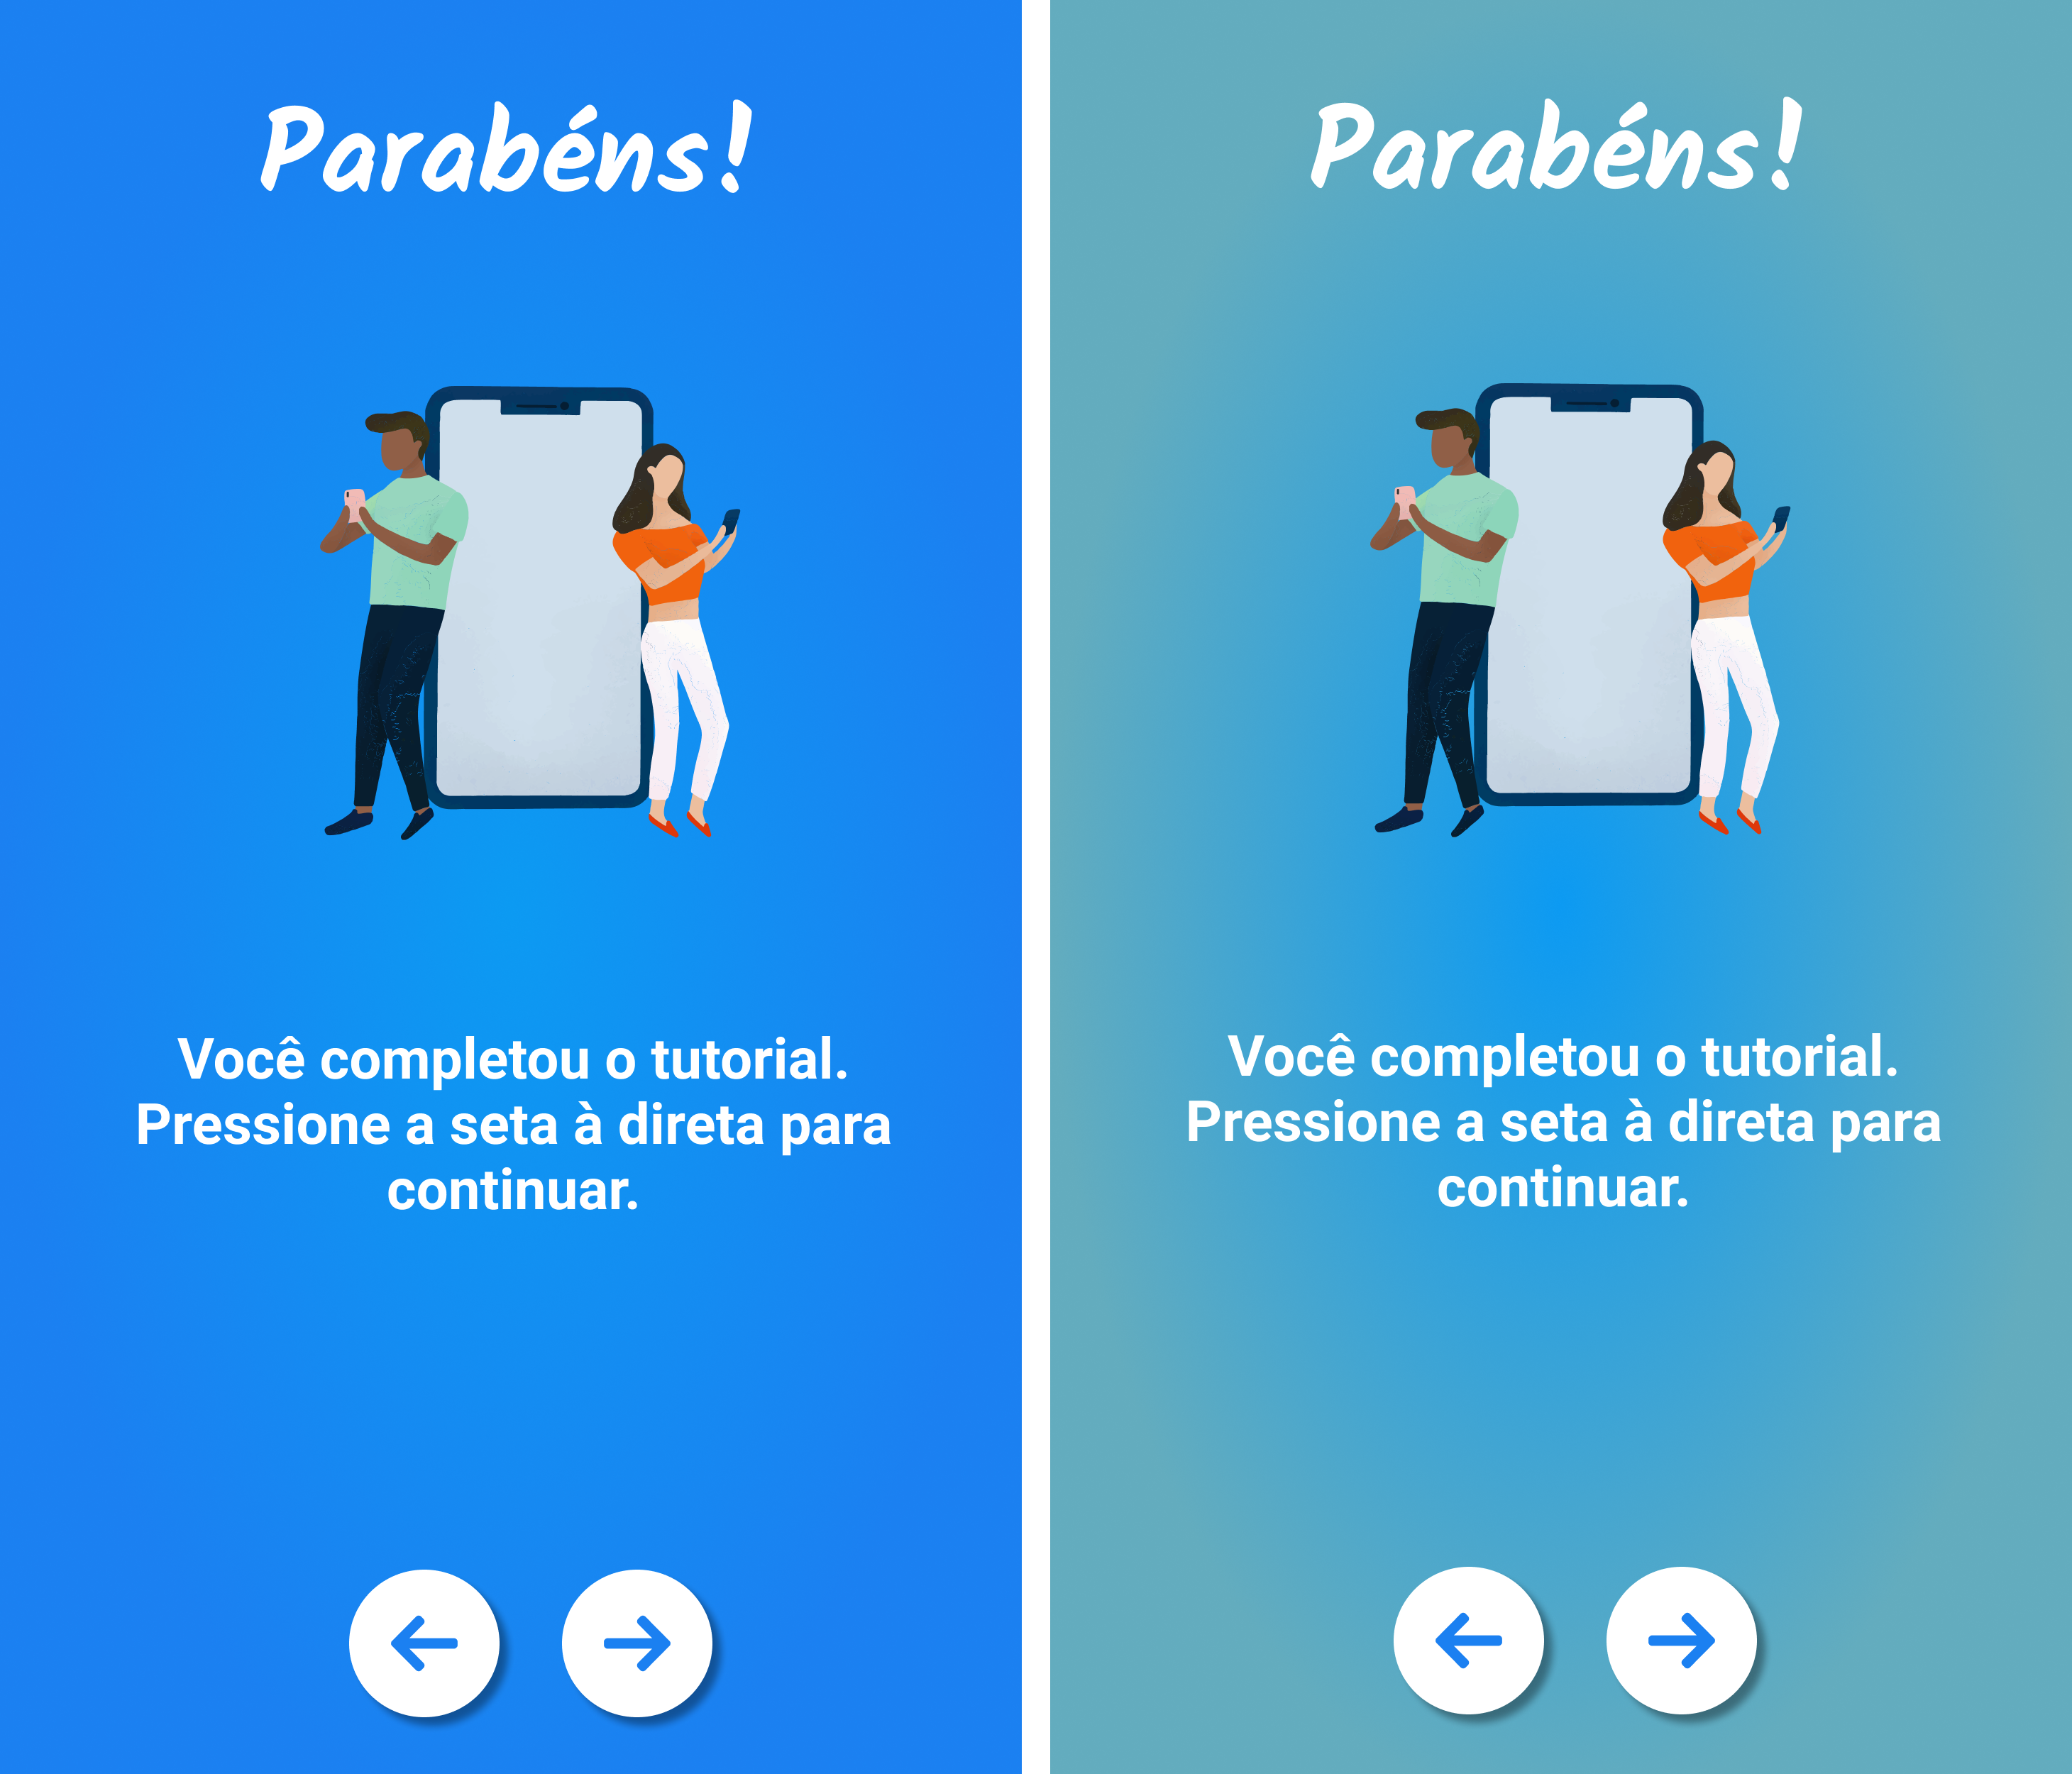
\includegraphics[width=0.9\textwidth]{Figuras/novascores.png}
    
    Fonte: Elaborada pelo autor
\end{figure}

Outra mudança foi a inserção do botão \textit{Home} no cabeçalho das telas. Dessa maneira é possível retornar à tela inicial a qualquer momento.

\begin{figure}[H]
\centering
    \caption{Novo cabeçalho com botão de voltar à tela inicial}
    \label{fig:botaohome}
    \includegraphics[width=0.9\textwidth]{Figuras/botaohome.png}
    
    Fonte: Elaborada pelo autor
\end{figure}

Foi criada uma tela para seleção de qual tipo de conteúdo o usuário aprenderá (Figura \ref{fig:selecaoconteudo}), não sendo mais obrigatório passar pelos três tipos.

\begin{figure}[H]
\centering
    \caption{Nova tela de seleção de tipo de conteúdo}
    \label{fig:selecaoconteudo}
    \includegraphics[width=0.4\textwidth]{Figuras/selecaoconteudo.png}
    
    Fonte: Elaborada pelo autor
\end{figure}

O formulário para registro de nova conta apresentava um problema que poderia confundir os usuários. Ao tentar criar uma conta com informação errada, por exemplo um email inválido, a caixa de inserção ficava vermelha. Todavia, ao tentar redigitar com um conteúdo válido a cor vermelha não desaparecia, somente ao clicar no botão de Registro. Isso poderia levar a entender que mesmo com a correção feita o conteúdo estivesse errado. Portanto, foi necessário verificar se o valor inserido estava vazio. Nas linhas 48 e 49 da Figura \ref{fig:onchangeemail}, é possível observar a análise: se o valor inserido for diferente de uma \textit{String} vazia, o estado de erro no email deve ser mudado para falso.

\begin{figure}[H]
\centering
    \caption{Função \textit{onChangeEmail(value)}}
    \label{fig:onchangeemail}
    \includegraphics[width=0.9\textwidth]{Figuras/onchangeemail.png}
    
    Fonte: Elaborada pelo autor
\end{figure}

Por fim, pode-se dizer que foi alcançado o objetivo final de aplicar as funcionalidades desejadas e estudadas na Seção \ref{sec:estudo_funcionalidades_apps} e exibidas na Tabela \ref{tab:funcionalidade}; com destaque para o aprendizado por áudio, teclado personalizado e conteúdo explicado por tutoriais.